%!TEX TS-program = xelatex

% Данный шаблон подготовлен для курса LaTeX в РАНХиГС
% на основе шаблона 
% Данила Фёдоровых (danil@fedorovykh.ru),
%  который использовал его в курсе 
% <<Документы и презентации в \LaTeX>> НИУ ВШЭ
% Исходная версия шаблона --- 
  % https://www.writelatex.com/coursera/latex/5.1
\documentclass[c, dvipsnames]{beamer}  % [t], [c], или [b] --- вертикальное 
%\documentclass[handout, dvipsnames, c]{beamer} % Раздаточный материал (на слайдах всё сразу)
% !TEX root = main_file.tex

%%%%%%%%%% Програмный код %%%%%%%%%%
% \usepackage{minted}
% Включает подсветку команд в программах!
% Нужно, чтобы на компе стоял питон, надо поставить пакет Pygments, в котором он сделан, через pip.

% Для Windows: Жмём win+r, вводим cmd, жмём enter. Открывается консоль.
% Прописываем pip install Pygments
% Заходим в настройки texmaker и там прописываем в PdfLatex или XelaTeX:
% pdflatex -shell-escape -synctex=1 -interaction=nonstopmode %.tex

% Для Linux: Открываем консоль. Убеждаемся, что у вас установлен pip командой pip --version
% Если он не установлен, ставим его: sudo apt-get install python-pip
% Ставим пакет sudo pip install Pygments

% Для Mac: Всё то же самое, что на Linux, но через brew.

% После всего этого вы должны почувствовать себя тру-программистами!
% Документация по пакету хорошая. Сам читал, погуглите!

%%%%%%%%%% Математика %%%%%%%%%%
\usepackage{amsmath,amsfonts,amssymb,amsthm,mathtools}
% Показывать номера только у тех формул, на которые есть \eqref{} в тексте.
%\mathtoolsset{showonlyrefs=true}
%\usepackage{leqno} % Нумерация формул слева

%%%%%%%%%% Шрифты %%%%%%%%%%
\usepackage[english, russian]{babel}   % выбор языка для документа
\usepackage[utf8]{inputenc}            % выбор utf8 кодировки
\usepackage[X2,T2A]{fontenc}           % ещё немного кодировки

\usepackage{fontspec}                  % пакет для подгрузки шрифтов
\setmainfont{Times New Roman}          % задаёт основной шрифт документа

\usepackage{unicode-math}              % пакет для установки математического шрифта
\setmathfont{Asana-Math.otf}           % шрифт для математики

% Конкретный символ из конкретного шрифта
% \setmathfont[range=\int]{Neo Euler}

%%%%%%%%%% Работа с картинками %%%%%%%%%%
\usepackage{graphicx}                  % Для вставки рисунков
\usepackage{graphics}
\graphicspath{{images/}{pictures/}}    % можно указать папки с картинками
\usepackage{wrapfig}                   % Обтекание рисунков и таблиц текстом


%%%%%%%%%% Работа с таблицами %%%%%%%%%%
\usepackage{tabularx}            % новые типы колонок
\usepackage{tabulary}            % и ещё новые типы колонок
\usepackage{array,delarray}      % Дополнительная работа с таблицами
\usepackage{longtable}           % Длинные таблицы
\usepackage{multirow}            % Слияние строк в таблице
\usepackage{float}               % возможность позиционировать объекты в нужном месте
\usepackage{booktabs}            % таблицы как в книгах
% Заповеди из документации к booktabs:
% 1. Будь проще! Глазам должно быть комфортно
% 2. Не используйте вертикальные линни
% 3. Не используйте двойные линии. Как правило, достаточно трёх горизонтальных линий
% 4. Единицы измерения - в шапку таблицы
% 5. Не сокращайте .1 вместо 0.1
% 6. Повторяющееся значение повторяйте, а не говорите "то же"
% 7. Есть сомнения? Выравнивай по левому краю!

%  вычисляемые колонки по tabularx
\newcolumntype{C}{>{\centering\arraybackslash}X}
\newcolumntype{L}{>{\raggedright\arraybackslash}X}
\newcolumntype{Y}{>{\arraybackslash}X}
\newcolumntype{Z}{>{\centering\arraybackslash}X}


%%%%%%%%%% Графика и рисование %%%%%%%%%%
\usepackage{tikz, pgfplots}    % язык для рисования графики из latex'a

%%%%%%%%%% Гиперссылки %%%%%%%%%%
\usepackage{xcolor}            % разные цвета

\usepackage{hyperref}
\hypersetup{
    unicode=true,           % позволяет использовать юникодные символы
    colorlinks=true,       	% true - цветные ссылки, false - ссылки в рамках
    urlcolor =blue,         % цвет ссылки на url
    linkcolor=black,        % внутренние ссылки
    citecolor=black,        % на библиографию
	breaklinks              % если ссылка не умещается в одну строку, разбивать ли ее на две части?
}

%%%%%%%%%% Другие приятные пакеты %%%%%%%%%%
\usepackage{multicol}       % несколько колонок
\usepackage{verbatim}       % для многострочных комментариев
\usepackage{enumitem}       % дополнительные плюшки для списков
%  например \begin{enumerate}[resume] позволяет продолжить нумерацию в новом списке

\usepackage{todonotes}      % для вставки в документ заметок о том, что  осталось сделать
% \todo{Здесь надо коэффициенты исправить}
% \missingfigure{Здесь будет Последний день Помпеи}
% \listoftodos --- печатает все поставленные \todo'шки

%%%%%%%%%%%%%%%%%%%%%%%%%%%%%%%%%%%%%%%%%%%
%%%%%%%%%% ГОСТОВСКИЕ ПРИБАМБАСЫ %%%%%%%%%%
%%%%%%%%%%%%%%%%%%%%%%%%%%%%%%%%%%%%%%%%%%%

% размер листа бумаги
\usepackage[paper=a4paper,top=15mm, bottom=15mm,left=35mm,right=10mm,includehead]{geometry}

% всякие разные расстояния
\usepackage{setspace}
\setstretch{1.33}              % Полуторный межстрочный интервал
\setlength{\parindent}{1.5em}  % Красная строка.

\righthyphenmin=2    % Разрешение переноса двух и более символов
\widowpenalty=10000  % Наказание за вдовствующую строку (одна строка абзаца на этой странице, остальное --- на следующей)
%\clubpenalty=10000  % Наказание за сиротствующую строку (омерзительно висящая одинокая строка в начале страницы)
\tolerance=1000      % Ещё какое-то наказание.

% Нумерация страниц сверху по центру
\usepackage{fancyhdr}
\pagestyle{fancy}
\fancyhead{ } % clear all fields
\fancyfoot{ } % clear all fields
\fancyhead[C]{\thepage}
% Чтобы не прорисовывалась черта!
\renewcommand{\headrulewidth}{0pt}

% Нумерация страниц с надписью "Глава"
\usepackage{etoolbox}
\patchcmd{\chapter}{\thispagestyle{plain}}{\thispagestyle{fancy}}{}{}

% Заголовки по левому краю
% опция identfirst устанавливает отступ в первом абзаце
\usepackage[indentfirst]{titlesec}{\raggedleft}

% В Linux этот пакет для заголовков. Исправляет это следующий непонятный кусок кода:
\makeatletter
\patchcmd{\ttlh@hang}{\parindent\z@}{\parindent\z@\leavevmode}{}{}
\patchcmd{\ttlh@hang}{\noindent}{}{}{}
\makeatother

% Редактирования Глав и названий
\titleformat{\chapter}
      {\normalfont\large\bfseries}
      {\thechapter }{0.5 em}{}

% Редактирование ненумеруемых глав chapter* (Введение и тп)
\titleformat{name=\chapter,numberless}
{\centering\normalfont\bfseries\large}{}{0.25em}{\normalfont}

% Убирает чеканутые отступы вверху страницы
\titlespacing{\chapter}{0pt}{-\baselineskip}{\baselineskip}

% Более низкие уровни (подзаголовки)
\titleformat{\section}{\bfseries}{\thesection}{0.5 em}{}
\titleformat{\subsection}{\bfseries}{\thesubsection}{0.5 em}{}

\titlespacing*{\section}{0 pt}{\baselineskip}{\baselineskip}
\titlespacing*{\subsection}{0 pt}{\baselineskip}{\baselineskip}

% Содержание, команды ниже изменяют отступы и рисуют точечки!
\usepackage{titletoc}

\titlecontents{chapter}
             [1em] %
             {\normalsize}
             {\contentslabel{1 em}}
             {\hspace{-1 em}}
             {\normalsize\titlerule*[10pt]{.}\contentspage}

\titlecontents{section}
              [3 em] %
              {\normalsize}
              {\contentslabel{1.75 em}}
              {\hspace{-1.75 em}}
              {\normalsize\titlerule*[10pt]{.}\contentspage}

\titlecontents{subsection}
              [6 em] %
              {\normalsize}
              {\contentslabel{3 em}}
              {\hspace{-3 em}}
              {\normalsize\titlerule*[10pt]{.}\contentspage}

% Правильные подписи под таблицей и рисунком
% Документация к пакету на русском языке!
\usepackage[tableposition=top, singlelinecheck=false]{caption}
\usepackage{subcaption}

   \DeclareCaptionStyle{base}%
		[justification=centering,indention=0pt]{}
   \DeclareCaptionLabelFormat{gostfigure}{Рисунок #2}
   \DeclareCaptionLabelFormat{gosttable}{Таблица #2}

   \DeclareCaptionLabelSeparator{gost}{~---~}
   \captionsetup{labelsep=gost}

   \DeclareCaptionStyle{fig01}%
           [margin=5mm,justification=centering]%
           {margin={3em,3em}}
   \captionsetup*[figure]{style=fig01,labelsep=gost,labelformat=gostfigure,format=hang}

   \DeclareCaptionStyle{tab01}%
           [margin=5mm,justification=centering]%
           {margin={3em,3em}}
   \captionsetup*[table]{style=tab01,labelsep=gost,labelformat=gosttable,format=hang}

% межстрочный отступ в таблице
 \renewcommand{\arraystretch}{1.2}

% многостраничные таблицы под РОССИЙСКИЙ СТАНДАРТ
% ВНИМАНИЕ! Обязательно после пакета caption!
\usepackage{fr-longtable}

%Более гибкие спсики
\usepackage{enumitem}

% сообщаем окружению о том, что существует такая штука, как нумерация русскими буквами
\makeatletter
\AddEnumerateCounter{\asbuk}{\russian@alph}{щ}
\makeatother

% ГОСТОВСКИЕ СПИСКИ

% Первый тип списков. Большая буква.
\newlist{Enumerate}{enumerate}{1}

\setlist[Enumerate,1]{labelsep=0.5em,leftmargin=1.25em,labelwidth=1.25em,
parsep=0em,itemsep=0em,topsep=0ex, before={\parskip=-1em},label=\arabic{Enumeratei}.}

% Второй тип списков. Маленькая буква.
\setlist[enumerate]{label=\arabic{enumi}),parsep=0em,itemsep=0em,topsep=0.75ex, before={\parskip=-1em}}

% Третий тип списков. Два уровня.
\newlist{twoenumerate}{enumerate}{2}
\setlist[twoenumerate,1]{itemsep=0mm,parsep=0em,topsep=0.75ex,, before={\parskip=-1em},label=\asbuk{twoenumeratei})}
\setlist[twoenumerate,2]{leftmargin=1.3em,itemsep=0mm,parsep=0em,topsep=0ex, before={\parskip=-1em},label=\arabic{twoenumerateii})}

% Четвёртый тип списков. Список с тире.
\setlist[itemize]{label=--,parsep=0em,itemsep=0em,topsep=0ex, before={\parskip=-1em},after={\parskip=-1em}}

% WARNING WARNING WARNIN!
% Если в списке предложения, то должна по госту стоять точка после цифры => команда Enumerate! Если идет перечень маленьких фактов, не обособляемых предложений то после цифры идет скобка ")" => команда enumerate! Если перечень при этом ещё и двууровневый, то twoenumerate.


%%%%%%%%%% Список литературы %%%%%%%%%%

%\usepackage[
%backend=biber, %подключение пакета biber (тоже нужен)
%bibstyle=gost-numeric, %подключение одного из четырех главных стилей biblatex-gost
%sorting=ntvy, %тип сортировки в библиографии
%]{biblatex}
\usepackage[backend=biber,style=gost-numeric, maxbibnames=9,maxcitenames=2,uniquelist=false, babel=other]{biblatex}

% Справка по 4 главным стилям для ленивых:
% gost-inline  ссылки внутри теста в круглых скобках
% gost-footnote подстрочные ссылки
% gost-numeric затекстовые ссылки
% gost-authoryear тоже затекстовые ссылки, но немного другие

% Подробнее смотри страницу 4 документации. Она на русском.

% Ещё немного настроек
\DeclareFieldFormat{postnote}{#1} %убирает с. и p.
\renewcommand*{\mkgostheading}[1]{#1} % только лишь убираем курсив с авторов

\addbibresource{bib.bib} 

% Этот кусок кода выносит русские источники на первое место. Костыль описали авторы пакета в руководстве к нему. Подробнее смотри:
% https://github.com/odomanov/biblatex-gost/wiki/Как-сделать%2C-чтобы-русскоязычные-источники-предшествовали-остальным
\DeclareSourcemap{
  \maps[datatype=bibtex]{
    \map{
      \step[fieldsource=langid, match=russian, final]
      \step[fieldset=presort, fieldvalue={a}]
    }
    \map{
      \step[fieldsource=langid, notmatch=russian, final]
      \step[fieldset=presort, fieldvalue={z}]
    }
  }
}

\DefineBibliographyStrings{english}{%
pages = {P\adddot},
number = {№},
}

\title[МСР в макроэкономике]{Оценка макроэкономических зависимостей с использованием методов снижения размерности в данных}
\subtitle{Отчёт по научно-исследовательской работе}


\author[Михаил Гареев]{Михаил Гареев \\ \smallskip \scriptsize ЭО-15-01 \\ \smallskip \scriptsize \href{mailto:mkhlgrv@gmail.com}{\nolinkurl{mkhlgrv@gmail.com} }}

\superviser{к.э.н. Полбин А.В.}

%\author[Имя автора]{Имя автора \\ \smallskip \scriptsize \href{mailto:author@ranepa.ru}{author@ranepa.ru} \\ \smallskip  \href{http://ranepa.ru}{http://ranepa.ru} }

\institute[РАНХиГС]{ \uppercase{
  Российская Академия Народного Хозяйства и  \\ Государственной Службы при Президенте Российской Федерации}}
\date{2018}


\titlegraphic{
\includegraphics[scale=0.5]{logo/logo_ranepa.png}}
\titlegraphicii{
\includegraphics[scale=0.5]{logo/logo_emit.png}}

\begin{document}

\frame[plain]{\titlepage}	% Титульный слайд


\begin{frame}[c]{Актуальность исследования} 
\begin{itemize}
\item  При оценке моделей из макроэкономики часто можно столкнуться с тем, что параметров относительно много, а наблюдений - мало. Иногда эту проблему решается использованием \alert{методов снижения размерности в данных}.
\end{itemize}
\end{frame}


% \begin{frame}[c]
% \frametitle{Анализ предметной области}
% { \small   % вместо small можно поставить scriptsize чтобы влезло
% 	\begin{table}[]
% 		\centering
% 		\resizebox{\textwidth}{!}{ 
%   			\begin{tabular}{|p{2.2cm}|p{1.8cm}|p{3.5cm}|p{7cm}|}
%   				\hline\rowcolor{backgr}
%   				\textcolor{white}{Авторы} & \textcolor{white}{Выборка, период}  & \textcolor{white}{Метод исследования}& \textcolor{white}{Результат} \\			
%   				\hline
%   				(Kuper, 2003)  & США, 998-2008  &  Коинтеграци и VECM & Получились значимые результаты с интересной интерпретацией.\\
%   				\hline
%   		\end{tabular} }
% 	\end{table}
% }
% \end{frame}


\begin{frame}[shrink=3]
	\frametitle{Цели и задачи}
	\begin{block}{Цель:}
	\begin{itemize}
		\item  Проверка некоторых гипотез макроэкономики при помощи методов
снижения размерности в данных и создание на их основе предсказательных моделей
для макроэкономических показателей.
	\end{itemize}
		
	\end{block}

	 	\begin{block}{Задачи:}
			\begin{enumerate}
	\item Обзор методов снижения размерности (LASSO, Post-LASSO, Dantzig Selector и др.).
\item Применение этих методов для оценки макроэкономических
зависимостей, анализ результатов, сравнение с другими методами оценивания и с
результатами, полученными ранее. 
\item Построение предсказательных моделей.
\item Создание процедуры мэтчинга стран на основе их макроэкономических показателей.
	 \end{enumerate}	
	\end{block}
\end{frame}



\section{Методы снижения размерности}
\subsection{Разреженная линейная модель с высокой размерностью в данных}

\begin{frame}
\frametitle{\insertsection} 
\framesubtitle{\insertsubsection}
Модель: 
  \begin{equation} 
\beta_0 + \varepsilon_i, \epsilon_i \sim N(0, \sigma^2), \beta_0 \in
\mathbb{R}^p, i = 1, \dots, n, 
\end{equation}
где:
  \begin{itemize}
\item $y_i$ --- это значения объясняемой
переменной, 
\item $x_i$ --- это значения $p$-размерной объясняющей переменной,
\item $\varepsilon_i$ --- значения независимых случайных ошибок в каждом наблюдении $i$, 
\end{itemize}
при этом возможно, что $p \geq n$, но только $s<n$ компонентов вектора$\beta_0$ не равны $0$.

\alert{Можно ли уменьшить размерность модели?}
\end{frame}

\subsection{Oracle Problem}
\begin{frame}[shrink=5]
\frametitle{\insertsection} 
\framesubtitle{\insertsubsection}
\begin{block}{Задача (Oracle Problem):}
\begin{equation}\label{op}
    \min_{\beta \in
\mathbb{R}^p} \mathbb{E}_n\left[ (y_i - {x_i}^{'} \beta)^2 \right] + \sigma^2
\frac{\left\lVert \beta \right\rVert_0}{n}, 
\end{equation} 
где $\left\lVert \beta \right\rVert_0$ --- это количество ненулевых компонентов в векторе $\beta$,  обобщение понятия нормы для степени $0$. 
\end{block}
\begin{block}{Гёльдерова норма для вектора $x$ степени $p$: }
\begin{equation}
    \left\lVert x \right\rVert_p = \sqrt[p]{\sum_i|x_i|^p},
\end{equation}
где обычно $p \geq 1$.

\end{block}

Решение \eqref{op} --- это  баланс между ошибкой регрессии и количеством ненулевых коэффициентов из вектора $\beta$. 

Методы снижения размерности оптимизируют эмпирические аналоги задачи \eqref{op}.
\end{frame}



\subsection{}



\begin{frame} 
\frametitle{\insertsection}  
\framesubtitle{\insertsubsection}
 	\begin{block}{AIC/ BIC}
  \begin{equation}
  \hat{\beta}  \in \arg \min_{\beta \in
\mathbb{R}^p} \sum_i=1^n \left[ (y_i - {x_i}^{'} \beta)^2 \right] +  \frac{\lambda}{n} \left\lVert \beta \right\rVert_0, 
\end{equation}
где $\lambda$ --- параметр штрафа.
 \end{block}

 \begin{block}{LASSO}
  \begin{equation}
  \hat{\beta}^{\text{LASSO}} \in \arg \min_{\beta \in
\mathbb{R}^p} \sum_i=1^n \left[ (y_i - {x_i}^{'} \beta)^2 \right] +  \frac{\lambda}{n} \left\lVert \beta \right\rVert_1,
\end{equation}
где $\lambda$ --- параметр штрафа, выбирается алгоритмически.
 \end{block}
 
\end{frame}

\begin{frame}
	\frametitle{\insertsection} 
\framesubtitle{\insertsubsection}

\begin{block}{Post-LASSO}
	\begin{enumerate}
		\item Использовать метода LASSO, найти $\hat{\beta}$.
		\item Применить МНК-регрессию, оценивая только неисключенные параметры $\beta$:
		\begin{equation}
		\tilde{\beta} \in \arg \min_{\beta \in
			\mathbb{R}^p} \sum_i=1^n \left[ (y_i - {x_i}^{'} \beta)^2 \right] +  \frac{\lambda}{n} \left\lVert \beta \right\rVert_1, \beta_j = 0| /hat{beta_j} = 0.
		\end{equation}
	\end{enumerate}
\end{block}


\begin{block}{Dantzig Selector}
	

\begin{eqnarray}
  \hat{\beta^{/text{DS}}} \min_{\beta \in
	\mathbb{R}^p} \left\lVert \beta \right\rVert_1\\
\text{s.t. } \left|x_i\beta - y_i\right| \leq \lambda \forall i = 1,\dots,n,
\end{eqnarray}

где $\lambda$ --- параметр штрафа, выбирается алгоритмически.

 \end{block}

\end{frame}

\section{Проверка гипотезы конвергенции с помощью методов снижения размерности}
\subsection{Однофакторная модель}
\begin{frame}
\frametitle{\insertsection} 
\framesubtitle{\insertsubsection}
    \begin{block}{Модель}
    \begin{equation}
g_i = \alpha +\beta ln(G_i) + \varepsilon_i, \epsilon_i \sim N(0, \sigma^2),
\end{equation}
где:
\begin{itemize}
    \item $g_i$ --- средний за 1980--1984 темп роста реального ВВП на душу населения, 
    \item $G_i$ --- логарифим ВВП на душу населения в 1980 г. (в долларах) для страны $i, i =1, \dots, 245$.
\end{itemize}
    \end{block}
    Данные:
    
\end{frame}


\section{Проверка гипотезы конвергенции с помощью методов снижения размерности.}
\subsection{Использование LASSO}
\begin{frame}
\frametitle{\insertsection} 
\framesubtitle{\insertsubsection}
    \begin{block}{Модель}
    \begin{equation}
g_i = \alpha +\beta ln(G_i) + \varepsilon_i, \epsilon_i \sim N(0, \sigma^2),
\end{equation}
где:
\begin{itemize}
    \item $g_i$ --- средний за 1980--1984 темп роста реального ВВП на душу населения, 
    \item $G_i$ --- логарифим ВВП на душу населения в 1980 г. (в долларах) для страны $i, i =1, \dots, 245$.
\end{itemize}
    \end{block}
    
    
\end{frame}
\subsection{Данные}
\begin{frame}
\frametitle{\insertsection} 
\framesubtitle{\insertsubsection}
    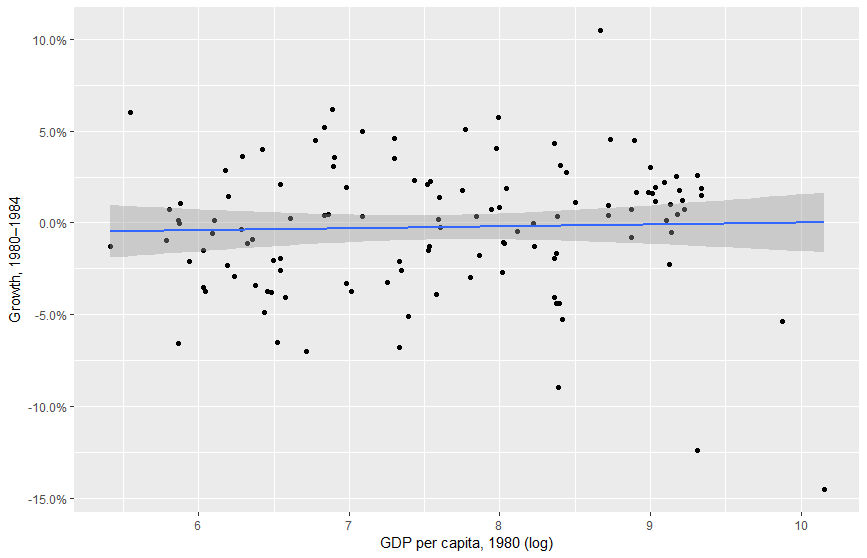
\includegraphics[width=\textwidth]{plot/gdp2growth_BL.png}
\end{frame}

\subsection{Сравнение результатов}
\begin{frame}
\frametitle{\insertsection} 
\framesubtitle{\insertsubsection}
{\scriptsize
\begin{table}[!htbp] \centering 
  \caption{Результаты регрессий} 
  \label{} 
\begin{tabular}{@{\extracolsep{5pt}}lcc} 
\\[-1.8ex]\hline 
\hline \\[-1.8ex] 
\\[-1.8ex] & \multicolumn{2}{c}{g} \\ 
\\[-1.8ex] & (1) & (2) \\ 
\hline \\[-1.8ex] 
 G & 0.001 ($-$0.005, 0.007) & $-$0.0112 ($-$0.022, 0.001) \\ 
  C & $-$0.010 ($-$0.055, 0.034) & $-$0.03 ($-$0.032, 0.041) \\ 
 \hline \\[-1.8ex] 
Наблюдений & 120 & 120 \\ 
R$^{2}$ & 0.001 & 0.001 \\ 
Adjusted R$^{2}$ & $-$0.007 & $-$0.007 \\ 
lambda & & 2.7870\\
\hline 
\hline \\[-1.8ex] 
\textit{Примечание:}  & \multicolumn{2}{r}{$^{*}$p$<$0.1; $^{**}$p$<$0.05; $^{***}$p$<$0.01} \\ 
\end{tabular} 
\end{table}
}


\end{frame}


\section{Краткий вывод и планы}
\begin{frame}
\frametitle{\insertsection} 
\begin{itemize}
    \item  Методы снижения размерности (LASSO, Post-LASSO и др.) потенциально представляют собой мощный инструмент для нахождения и проверки макроэкономических зависимостей.
    \item Планы на ближайшее время:
    \begin{itemize}
        \item  Сделать осмысленные LASSO, Post-Lasso регрессии для проверки гипотезы конвергенции на основе современных данных Всемирного банка.
        \item Проверить другие макроэкономические гипотезы с помощью методов снижения размерности.
    \end{itemize}
\end{itemize}
   
    
\end{frame}



\begin{frame}[c, plain]
\begin{center}

{\LARGE Спасибо за внимание}

\bigskip

{\Large \inserttitle}

\bigskip

{\insertauthor} 

\bigskip

\bigskip\bigskip

{\large \insertdate}
\end{center}
\end{frame}



\begin{frame}[c, plain]
  \frametitle{Источники}    
  \begin{thebibliography}{10}    
  \beamertemplatearticlebibitems
  \bibitem{ch1}
    Belloni, Alexandre and Chernozhukov, Victor
    \newblock High dimensional sparse econometric models: An introduction.
    \newblock Springer, 2011
   \bibitem{ch2}
   Belloni, Alexandre, Victor Chernozhukov, and Christian Hansen. 
   \newblock Lasso methods for gaussian instrumental variables models
   \newblock 2011
    \bibitem{bl}
    Barro, Robert J.  and Lee, Jong-Wha 
    \newblock Data Set for a Panel of 138 Countries
    \newblock 1994
    \bibitem{g}
     Candes, Emmanuel, and Terence Tao. 
    \newblock The Dantzig selector: Statistical estimation when p is much larger than n.
    \newblock The Annals of Statistics 35.6 (2007): 2313-2351.
    \bibitem{f}
     Akaike, Hirotugu.
    \newblock A new look at the statistical model identification.
    \newblock IEEE transactions on automatic control 19.6 (1974): 716-723.
  \end{thebibliography}
\end{frame}




\end{document}